% =====================================================================
%  Introduction à la thermique du bâtiment pour les architectes
%  Projet principal : ne contient que la structure du livre.
%  Le contenu est dans le dossier parties/ (un fichier par partie).
% =====================================================================
\documentclass[11pt,a4paper,oneside,openany]{book}
% =====================================================================
%  Préambule : packages et réglages communs.
%  Restez sur des packages courants : ceux-ci sont tous compris
%  par la version web du cours.
% =====================================================================
\usepackage[utf8]{inputenc}
\usepackage[T1]{fontenc}
\usepackage[french]{babel}
\usepackage{lmodern}
\usepackage[margin=2.5cm]{geometry}
\usepackage{amsmath,amssymb,amsthm}
\usepackage{graphicx}
\usepackage[hidelinks]{hyperref}

% Numérotation des équations et figures par chapitre : (1.1), (1.2)…
\numberwithin{equation}{chapter}

% Exercices et corrigés
% Sur le site, « exercice » devient un encadré et « corrige » un encadré dépliable.
\theoremstyle{definition}
\newtheorem{exercice}{Exercice}[chapter]
\newtheorem*{corrige}{Corrigé}

% Vos macros
\newcommand{\unite}[1]{\,\mathrm{#1}}


\title{Introduction à la thermique du bâtiment pour les architectes}
\author{Victor De Bono}
\date{ENSAP Lille, A321 Ambiances\\ \today}

\begin{document}

\frontmatter
\maketitle

\mainmatter
\tableofcontents

\newpage
\part{Introduction générale}
\chapter{Introduction et objectifs}
\label{chap:introduction}

\section{Présentation du cours}
Ce document est le support de cours de l'enseignement A321 Ambiances, dispensé à l'ENSAP Lille. Il ne se substitue pas au cours : il en est plutôt un résumé synthétique. En effet, sans explications orales, ce cours peut paraître \textit{trop technique} pour une licence d'architecture, de par les nombreuses équations et unités utilisées. J'insiste sur le fait que le cours est tout à fait accessible : il est possible de le comprendre sans avoir de bagage mathématique. Les équations sont toujours expliquées en cours. De plus, les concepts présentés dans ce cours sont faits pour être compris puis manipulés par les architectes, sans en faire de futurs physiciens. Ainsi, des conclusions sont présentées en fin de chaque chapitre et récapitulent les informations essentielles qui seront à mobiliser en projet. Pour conclure : la lecture de ce cours peut paraître austère, elle représente uniquement la partie synthétique d'un cours magistral qui lui est beaucoup plus vivant et pédagogique.

\textbf{Ce document est en cours d'élaboration et fait suite à la lutte de 2026 dans les ENSA, il n'est pas encore finalisé (il manque notamment de nombreuses figures): il peut donc contenir des erreurs. Si vous repérez des erreurs merci de me les faire remonter.}

Dernières mise à jour : \today.
\\

Ce cours est composé de 7 Parties principales :
\begin{itemize}
  \item \textbf{Partie 1 : Introduction générale.} Cette partie présente le cours et ses objectifs, puis pose les notions de base : énergie, température, chaleur et propriétés thermiques des matériaux.

  \item \textbf{Partie 2 : Transferts de chaleur.} Cette partie est consacrée au passage de la chaleur à travers ses trois modes : la conduction, la convection et le rayonnement. Pour chaque mode, son fonctionnement est présenté ainsi que sa traduction dans le bâtiment

  \item \textbf{Partie 3 : Transferts de vapeur.} Cette partie s'intéresse à l'humidité de l'air : pression de vapeur, diagramme de l'air humide, migration de la vapeur d'eau à travers les parois et risques de condensation.

  \item \textbf{Partie 4 : Climat.} Cette partie élargit pour dézoomer  à l'échelle du globe : effet de serre, entrée dans l'Anthropocène et dérèglement climatique, pour comprendre le contexte dans lequel s'inscrit aujourd'hui la conception architecturale.

  \item \textbf{Partie 5 : Thermique architecturale.} Cette partie revient au projet. Elle aborde le comportement du bâtiment en régime dynamique, le rôle de l'enveloppe, la notion de confort (d'hiver et d'été), ainsi que les équipements courant des bâtiments : ventilation, chauffage et climatisation.

  \item \textbf{Partie 6 : Cadre réglementaire.} Cette partie retrace l'évolution de la réglementation thermique française, actuellement en vigueur, la RE 2020, à travers ces trois volets : carbone, énergie et confort d'été.

  \item \textbf{Partie 7 : Conclusion générale.} Cette dernière partie fait la synthèse du cours. Elle propose des pistes d'intervention en projet neuf comme en réhabilitation, et des ressources pour aller plus loin.
\end{itemize}

\section{Objectifs pédagogiques}
L'ensemble des parties d'un bâtiment est soumis aux transferts thermiques, 
qui sont des échanges de chaleur entre un milieu chaud et un milieu froid : La connaissance et la maîtrise de ces transferts thermiques permet d’influer sur le confort des usagers et de gérer la facture énergétique d'un bâtiment.

Les objectifs de ce cours sont de :
\begin{itemize}
    \item Comprendre les phénomènes physique qui sont à l’œuvre dans les transferts de chaleurs et de vapeurs.
    \item Être capable de comprendre le rôle des différents matériaux au sein de l'enveloppe du bâtiment
    \item Établir des stratégies de conception et/ou de réhabilitation pour assurer le confort des usagers (en hiver et en été)
    \item Connaître les réglementations en vigueurs dans le secteur de l'architecture sur la thermique, l’énergie et l'environnement.

\end{itemize}

\section{Références}
La bibliographie complète est présente en fin de cours. Ce cours est en grande partie inspiré de quatre sources principales :
\begin{itemize}
    \item Des cours de thermique dispensés à l'ENSAB par Pierre Antoine Chabriac
    \item Du \textit{Manuel de performance énergétique du bâtiment} de Simon Rouchier \footfullcite{rouchier-manuel}
    \item Du livre \textit{La Thermique du Bâtiment} d'Olivier Benjeddou \footfullcite{benjeddou-thermique}.
    \item Du site Énergie plus \footfullcite{energieplus}
\end{itemize}
\chapter{Historique, concepts et unités}
\label{chap:concepts}

% ---------------------------------------------------------------------
\section{Énergie}

\subsection*{Énergie, usage courant}
L'énergie est un concept dont il peut être complexe de donner une définition, On parle d'énergie dans de nombreux domaines (physique, philosophie, ésotérisme, etc.) avec des définitions variables, et parfois même divergentes.

\subsection*{Énergie, en physique (thermodynamique)}
\textbf{L'énergie désigne la capacité à effectuer des transformations}, c'est-à-dire à modifier l'état d'un système\footfullcite{klein-energie}.

\textbf{L'énergie est ce qui quantifie le changement d'état d'un système}\footfullcite{jancovici2019}. Par exemple :
\begin{itemize}
  \item une modification de température (un radiateur qui chauffe) ;
  \item une modification de vitesse (un bus qui se déplace) ;
  \item une modification de forme (une pelleteuse qui creuse).
\end{itemize}
% [Figure : radiateur / bus / pelleteuse]

L'énergie est le travail d'une force et se mesure en joules (J).
1 joule est défini comme le travail d'une force d'un newton qui se déplace d'un mètre dans la direction de la force :
\begin{equation}
  1\,\mathrm{J} = 1\,\mathrm{N}\times\mathrm{m} = 1\,\mathrm{kg\cdot m^2/s^2} = 1\,\mathrm{kg\cdot m^{2}\cdot s^{-2}}
\end{equation}


D'autres unités ont pu être utilisées par le passé, par exemple la calorie (cal).
1 calorie est définie comme l'énergie nécessaire pour élever la température d'un gramme d'eau liquide de 1\,°C :
\begin{equation}
  1\,\mathrm{cal} \simeq 4{,}2\,\mathrm{J}
\end{equation}


\subsection*{Énergie, en physique (thermodynamique) appliquée au bâtiment}
On utilisera davantage le watt-seconde (W.s) ou le kilowatt-heure (kWh) qui sont des dérivés du joule.

Le watt est une unité de puissance : c'est-à-dire le transfert d'énergie au cours du temps.
Le watt (W) représente la puissance d'un système dans lequel une énergie d'un joule est transférée uniformément pendant une seconde :
\begin{equation}
  1\,\mathrm{W} = 1\,\mathrm{J/s} = 1\,\mathrm{kg\cdot m^2/s^3} = 1\,\mathrm{kg\cdot m^{2}\cdot s^{-3}}
\end{equation}

La quantité de chaleur $Q$ (J) dépend du temps $t$ (s) et de la puissance thermique $P$ (W) :
\begin{equation}
  P = \frac{Q}{t}
\end{equation}

On peut donc définir le watt-heure (Wh) tel que : $1\,\mathrm{Wh} = 3600\,\mathrm{J}$ ou encore $1\,\mathrm{kWh} = 3600\,\mathrm{kJ}$.

\subsection*{Conservation de l'énergie}
L'énergie désigne la capacité à effectuer des transformations.
La quantité d'énergie d'un système fermé reste fixe tant qu'il n'y a pas de transformation : \textbf{l'énergie est une grandeur qui se conserve}\footfullcite{planck1887}.

\begin{itemize}
  \item On ne produit pas de l'énergie : on transforme la forme qu'elle prend ou on la transfère.
  \item On ne consomme pas de l'énergie : on transforme la forme qu'elle prend ou on la transfère.
\end{itemize}

% ---------------------------------------------------------------------
\section{Température}

\subsection*{La température et la chaleur sont deux notions différentes}
\textbf{La température est la conséquence de l'excitation des particules composant la matière.}
\begin{itemize}
  \item Plus ces particules sont excitées, plus la matière est chaude.
  \item Cette excitation peut évoluer dans le temps, on observe alors une variation de température de la matière.
  \item Le corps humain a la capacité de sentir des variations infimes de température.
  \item En physique, on considère la température comme une variable dite « d'état » car elle caractérise un état de la matière et non une évolution.
\end{itemize}

\subsection*{L'humain et la perception de la température}
l'etre humain possède des themorecepteurs capable de ressentir des petites variations de températures. Ces thermorécepteurs sont des terminaisons nerveuses mesurant la température cutanée \footfullcite{livrescolaire-thermorecepteurs}.
Il existe deux types de thermorécepteurs :
\begin{itemize}
  \item les thermorécepteurs au « chaud » (entre 30 et 44\,°C) ;
  \item les thermorécepteurs au « froid » (entre 17 et 30\,°C).
\end{itemize}
La sensation thermique devient douloureuse si la température cutanée est inférieure à 17\,°C ou supérieure à 44\,°C : les neurones nociceptifs prennent le relais.
% [Figure : coupe de la peau]

\subsection*{Mesure de la température}
Historiquement plusieurs unités et echelles ont été proposé pour mesurer la température,

\subsubsection*{Le degré Celsius (°C)}
Le degré Celsius est une echelle de température proposée par Anders Celsius en 1742\footfullcite{beckman1997}. Son échelle est initialement définie par deux points :
  \begin{itemize}
    \item le point bas 0\,°C correspond à la température de solidification de l'eau (au niveau de la mer : à pression « standard ») ;
    \item le point haut 100\,°C correspond à la température d'ébullition de l'eau (au niveau de la mer : à pression « standard ») ;
    \item l'intervalle est divisé en 100.
  \end{itemize}

L'échelle Celsius est couramment utilisée dans le monde, et a été redéfinie pour s'aligner sur le \textbf{Système international d'unités}.
  

\subsubsection*{Le kelvin (K)}
Le Kelvin est proposé par William Thomson, (connu sous le nom de Lord Kelvin), en 1848\footfullcite{thomson1848} le Kelvin \textbf{Utilise la notion de zéro absolu} :
  \begin{itemize}
    \item le 0\,K correspond à la température la plus basse qui puisse exister (lorsque les particules ne sont pas excités du tout) ;
    \item l'intervalle est le même que celui de l'échelle des °C.
  \end{itemize}
Le kelvin est l'unité officielle du Système international d'unités, on l'utilise couramment en physique. C'est une grandeur qui sera donc toujours positive.


\subsubsection*{Conversion degré Celsius en kelvin}
\[
  0\,\mathrm{K} = -273{,}15\,^{\circ}\mathrm{C}
\]
L'intervalle est le même que celui de l'échelle des °C, ainsi :
\begin{equation}
  T(\mathrm{K}) = T(^{\circ}\mathrm{C}) + 273{,}15
\end{equation}
Pour convertir des degrés Celsius en kelvins, il suffit donc d'ajouter 273,15 à la température considérée.
Par exemple, 37\,°C = 310,15\,K.

% ---------------------------------------------------------------------
\section{Chaleur}

\textbf{La chaleur est une énergie} (elle s'exprime donc en J ou en kWh).
La chaleur est la quantité d'énergie qu'il faut apporter (ou ôter) afin de modifier la température de la matière.

Rappel : 1 calorie est définie comme l'énergie nécessaire pour élever la température d'un gramme d'eau liquide de 1\,°C ($1\,\mathrm{cal} \simeq 4{,}2\,\mathrm{J}$).

\textbf{La chaleur est l'énergie échangée lors d'un transfert thermique.}
% [Figure : l'exemple du welsh]

On distingue deux types de chaleurs : la chaleur sensible et la chaleur latente.

\subsection*{La chaleur sensible}
La chaleur sensible est la chaleur qui provoque une modification de la température d'un objet sans modifier son état.
Par exemple :
\begin{itemize}
  \item si on chauffe de l'eau de 25,°C à 70\,°C, la température monte au fur et à mesure que de la chaleur y est ajoutée sans que l'état de l'eau change : la hausse de chaleur est appelée chaleur sensible ;
  \item de la même manière, quand de la chaleur est enlevée d'un objet et que sa température baisse, la chaleur retirée est également appelée chaleur sensible.
\end{itemize}
\textbf{La chaleur sensible modifie la température d'une matière.}

\subsection*{La chaleur latente}
La chaleur latente est la chaleur qui provoque une modification d'état de la matière.
\begin{itemize}
  \item Tous les corps purs sont capables de modifier leur état.
  \item Les solides peuvent se liquéfier et les liquides peuvent devenir des gaz.
  \item Ces transformations nécessitent l'ajout ou le retrait de chaleur.
  \item La chaleur latente n'affecte pas la température d'une substance (l'eau reste à 100\,°C quand elle bout).
  \item La chaleur ajoutée pour maintenir l'eau en ébullition est la chaleur latente.
\end{itemize}
\textbf{La chaleur latente modifie l'état physique d'une matière.}


Une substance peut changer d'état physique de plusieurs façons, il existe donc plusieurs chaleurs latentes :
\begin{itemize}
  \item chaleur latente de fusion : quantité de chaleur pour passer de l'état solide à l'état liquide ;
  \item chaleur latente de vaporisation : quantité de chaleur pour passer de l'état liquide à l'état gazeux ;
  \item chaleur latente de liquéfaction (ou de condensation) : quantité de chaleur pour passer de l'état gazeux à l'état liquide ;
  \item chaleur latente de solidification : quantité de chaleur pour passer de l'état liquide à l'état solide.
\end{itemize}
% [Figure : courbe récapitulative chaleur sensible / chaleur latente]

% ---------------------------------------------------------------------
\section{Propriétés des matériaux}

\subsection*{Masse volumique}
C'est le rapport entre la masse (kg) d'un matériau et un volume donné (m$^3$). Son expression est donc :
\begin{equation}
  \rho = \frac{m}{V} \quad \mathrm{(kg/m^3)}
\end{equation}
On parlera également de densité $d$, qui est le rapport de la masse volumique d'un matériau à celle d'une référence, en général l'eau ($\rho = 1000$\,kg/m$^3$).

\subsection*{Conductivité thermique}
La conductivité thermique, notée $\lambda$, est la quantité d'énergie traversant 1\,m$^2$ de matériau d'un mètre d'épaisseur soumis à une différence de 1 degré de température. Elle s'exprime en $\mathrm{W\cdot m^{-1}\cdot K^{-1}}$ ou (W/m.K).

La conductivité themrique, $\lambda$ traduit la capcité d'un matériau à laisser passer ou non la chaleur. C'est une caractéristique intrinsèque et propre à chaque matériaux.
\begin{itemize}
    \item Plus la conductivité est faible, moins la matériau laisse passer la chaleur : il est donc un isolant thermique.
    \item Plus la conductivité est forte, plus le matériaux laisse passer la chaleur, c'est donc un conducteur thermique
\end{itemize}
  
Quelques références\footnote{\texttt{https://fr.wikipedia.org/wiki/Conductivit\%C3\%A9\_thermique}} sont consultables sur le web.

\subsection*{Capacité thermique}
La capacité thermique (ou capacité calorifique), notée $c$, d'un matériau quantifie la possibilité d'absorber ou de restituer de l'énergie par échange thermique.

\textbf{La capacité thermique est la chaleur qu'il faut transférer à un corps pour augmenter sa température d'un kelvin.} Elle s'exprime en J/K ($\mathrm{J\cdot K^{-1}}$).

On parle de capacités calorifiques :
\begin{itemize}
  \item massique, pour 1\,kg de matériau : $\displaystyle C_m = \frac{c}{m}$ \quad (J/kg.K) ;
  \item volumique, pour 1\,m$^3$ de matériau : $\displaystyle C_v = \frac{c}{V}$ \quad (J/m$^3$.K).
\end{itemize}

Quelques références\footnote{\texttt{https://fr.wikipedia.org/wiki/Capacit\%C3\%A9\_thermique\_massique}} sont consultables sur le web.

\subsubsection{différence entre conductivité et capacité thermqiue,}
Pour distinguer la différence entre conductivité et capacité, nous pouvons envisager l'analogie suivante: un réservoir d'eau alimenté par un tuyau.

si on assimile la température au niveau d'eau dans le reservoir, l'énergie échangée peut être assimilée au volume d'eau transféré et la puissance thermique au débit d'eau.

\begin{itemize}
  \item \textbf{$\lambda$ représente la résistance du tuyau.}
  Plus le tuyau est étroit, plus sa  conductivité est faible, le débit sera plus faible.

  \item \textbf{$C$ correspond à la surface horizontale du réservoir.}
  Plus le réservoir est large, plus il faut ajouter d'eau pour faire monter son niveau d'un centimètre.
  De même, une grande capacité thermique demande davantage d'énergie pour augmenter la température d'un degré.
\end{itemize}

\textbf{La conductivité désigne l’opposition d’un matériau au passage de la chaleur, tandis que la capacité thermique représente la quantité d’énergie que ce matériau (et peut restituer) pour augmenter sa température.}

% =====================================================================
\part{Transferts de chaleur}
% =====================================================================

\chapter{Conduction}
\label{chap:conduction}

\section{Mécanisme de la conduction}

\section{Loi de Fourier}
\label{sec:fourier}



\section{Conduction dans les parois}

\section{Ponts thermiques}

\section{Isolation}

\section{Exercices}

\chapter{Convection}
\label{chap:convection}

\section{Mécanisme de la convection}

\section{Convection naturelle et convection forcée}

\section{Convection dans le bâtiment}

\chapter{Rayonnement}
\label{chap:rayonnement}

\section{Mécanisme du rayonnement}

\subsection{Le Soleil}

\subsection{Les ondes électromagnétiques}

\section{Apports solaires}

\section{Rayonnement dans le bâtiment}

\chapter{Conclusion sur les transferts de chaleur}

% =====================================================================
%  Partie 3 -- Transferts de vapeur
% =====================================================================
\part{Transferts de vapeur}

\chapter{Transferts de vapeur}
\label{chap:vapeur}

\section{Introduction}

\subsection*{La vapeur d'eau}
L'eau peut passer d'un état à l'autre :
\begin{itemize}
  \item solide $\rightarrow$ liquide : fusion ; liquide $\rightarrow$ solide : solidification ;
  \item liquide $\rightarrow$ gaz : vaporisation ; gaz $\rightarrow$ liquide : liquéfaction ;
  \item solide $\rightarrow$ gaz : sublimation ; gaz $\rightarrow$ solide : condensation.
\end{itemize}
% [Figure : diagramme des changements d'état]

\subsection*{Le point triple de l'eau}
Le point triple de l'eau se situe à 0,01\,°C et environ 6\,mbar. À la pression atmosphérique (1013\,mbar), le point de fusion est à 0\,°C et le point d'ébullition à 100\,°C.
% [Figure : diagramme de phase de l'eau]

\subsection*{L'évaporation}
L'eau s'évapore au contact de l'air sans être à 100\,°C.
On estime en extérieur l'évaporation d'un plan d'eau entre 1\,mm et 10\,mm par jour en fonction des conditions météorologiques\footnote{M.E. Jensen, \emph{Estimating evaporation from water surfaces}, 2010.}.

Pour s'évaporer, l'eau doit changer d'état.
Elle absorbe l'énergie thermique de sa surface hôte pour s'évaporer.
Cette énergie est la chaleur latente.

\subsection*{La condensation}
% [Figures : bouteille froide, rosée, vitre, moisissures]

\section{Pression de vapeur et humidité}

\subsection*{Pression de vapeur}
Dans le cas de l'air humide, on appelle pression de vapeur, $p_v$, la pression (dite partielle) de la vapeur contenue dans l'air.
La pression de vapeur reflète la proportion de vapeur d'eau contenue dans l'air.

\subsection*{Pression de vapeur saturante}
La pression de vapeur saturante, $p_{vs}$, est la pression à laquelle la phase gazeuse est en équilibre avec sa phase liquide ou solide à une température donnée.
À l'équilibre, l'eau se rassemblera sous forme de gouttelettes sphériques pour équilibrer les forces en présence.
\begin{itemize}
  \item C'est la frontière à laquelle un gaz se changera en liquide ou en solide.
  \item La pression de vapeur saturante dépend de la température.
\end{itemize}

\subsection*{Humidité relative}
L'humidité relative de l'air, HR, ou degré hygrométrique, correspond au rapport de la pression partielle de vapeur d'eau contenue dans l'air sur la pression de vapeur saturante à la même température.

L'humidité relative est analogue à une mesure du rapport entre le contenu en vapeur d'eau de l'air et sa capacité maximale à en contenir dans ces conditions de température.
Ce rapport changera si on change la température.
L'humidité relative s'exprime en pourcentage :
\begin{equation}
  HR = \frac{p_v}{p_{vs}(T)} \times 100
\end{equation}
$p_{vs}$ peut se trouver dans des abaques dans lesquels elle est déjà calculée ou mesurée pour plusieurs températures.

Plus l'air est chaud, plus il peut contenir d'eau sous forme de vapeur.
Inversement, quand l'air se refroidit, la vapeur se condense et forme des gouttelettes d'eau liquide : on dit que le seuil de saturation augmente avec la température.

\subsection*{Diagramme de l'air humide}
Le diagramme de l'air humide permet de relier la température à la pression de vapeur saturante.
Par exemple, l'air à 20\,°C et 50\,\% d'humidité relative condense autour de 9\,°C.
% [Figures : diagramme de l'air humide (pression atmosphérique 101325 Pa), lecture du point de rosée, zone de confort]

\section{Passage de la vapeur}

\subsection*{Matériaux perspirants}
Les matériaux perspirants sont des matériaux qui permettent la diffusion de la vapeur d'eau.

Chaque matériau offre une certaine résistance à la migration de la vapeur d'eau ; cette résistance s'exprime par :
\begin{itemize}
  \item le coefficient de résistance à la diffusion de vapeur d'eau : $\mu$ (sans unité) ;
  \item la résistance à la diffusion de vapeur d'eau : $S_d$ (en mètres).
\end{itemize}

\subsection*{Coefficient de résistance à la diffusion de vapeur d'eau}
Le coefficient de résistance à la diffusion de vapeur $\mu$ représente la capacité d'un matériau à s'opposer au passage de la vapeur.

C'est une grandeur relative résultant du rapport entre la perméabilité à la vapeur d'eau de l'air et celle du matériau.
Plus $\mu$ est élevé, plus la résistance est élevée ($\mu$ est infini pour un métal et vaut 1 pour l'air).

La détermination du facteur de résistance à la diffusion de la vapeur dans un matériau est réalisée suivant un protocole défini dans la norme NF EN ISO 12572.

\subsection*{Résistance à la diffusion de vapeur d'eau}
La quantité de vapeur d'eau diffusant à travers une couche de matériau dépend aussi de l'épaisseur.
On appelle alors épaisseur équivalente de diffusion, $S_d$, la résistance qu'offre une couche de matériau à la diffusion de vapeur pour une épaisseur donnée.

$S_d$ est le produit de l'épaisseur $e$ d'un matériau et du coefficient de résistance à la diffusion de vapeur $\mu$ :
\begin{equation}
  S_d\ \mathrm{[m]} = \mu \times e\ \mathrm{[m]}
\end{equation}

Le $S_d$ d'une couche de matériau correspond à l'épaisseur en mètres de la couche d'air stationnaire qui exercerait la même résistance à la diffusion de vapeur que la couche de matériau.
Exemple : lorsque le $S_d$ d'un matériau vaut 5, cela signifie que cette couche de matériau équivaut à 5 mètres d'air stationnaire.

Le coefficient de résistance à la diffusion de vapeur de certains matériaux dépend de leur état : sec ou humide.

\subsection*{Frein-vapeur, pare-vapeur et pare-pluie}
Le \textbf{frein-vapeur} est un film fin qui freine le passage de la vapeur d'eau (murs perspirants). Il aura un $S_d$ de 1 à 5\,m.

On parle de frein-vapeur « intelligent » lorsque la membrane du frein-vapeur est à diffusion variable. Elle est alors composée de pores qui s'ouvrent ou se ferment en fonction de l'humidité de l'air : elle peut être frein-vapeur ou pare-vapeur.

Le \textbf{pare-vapeur} empêche le passage de la vapeur d'eau ; il se place du côté intérieur de l'habitation et possède un $S_d > 10$\,m.

Remarque : le \textbf{pare-pluie} se posera sous toiture ou à l'extérieur du mur. Son rôle est d'assurer l'étanchéité à l'eau, mais il doit laisser passer la vapeur d'eau.
Le $S_d$ d'un pare-pluie est de l'ordre de 0,18\,m.

\subsection*{Condensation de surface}
L'air intérieur peut arriver en contact avec une surface de température plus faible. Au contact, l'air se refroidit et la température qu'il atteint dans le voisinage de la surface peut se retrouver en dessous du point de rosée.
Il apparaît alors de la condensation dite \textbf{de surface} (la pression de vapeur dans l'air atteint la pression de saturation).
% [Figures : moisissures en angle]

Pour empêcher la condensation de surface, il faut :
\begin{itemize}
  \item avoir une qualité suffisante de l'isolation de l'enveloppe, de façon à ce que la température de la face intérieure de celle-ci ne descende pas en dessous de 17,5\,°C ;
  \item diminuer, par une ventilation complémentaire, l'humidité relative de l'air intérieur ;
  \item chauffer la face intérieure des parois froides.
\end{itemize}
Si ces mesures ne sont pas applicables ou sont insuffisantes, la seule façon de limiter les dégâts est de traiter la surface des parois pour empêcher la pénétration de l'eau de condensation par capillarité dans les parois, et de pouvoir recueillir et évacuer l'eau condensée.

\subsection*{Condensation interne}
La condensation interne se produit si, à un endroit d'un élément, la pression de vapeur réelle devient égale à la pression de saturation régnant à cet endroit.
Ce phénomène résulte des différences de pression de vapeur et de température.

Il existe bien souvent une différence de pression de vapeur entre l'intérieur et l'extérieur (production de vapeur par les occupants, les plantes, la lessive, la cuisson, le nettoyage).

En hiver, la pression partielle de vapeur intérieure est, en général, supérieure à celle correspondant au climat extérieur, et on a alors un flux de vapeur qui se produit.

Fonctionnement :
\begin{itemize}
  \item En hiver, la pression de vapeur est souvent plus élevée à l'intérieur qu'à l'extérieur.
  \item Ce différentiel de pression de vapeur engendre une migration de vapeur par diffusion vers l'extérieur.
  \item Au fur et à mesure qu'elle traverse les différents matériaux constituant l'enveloppe, la vapeur se rapproche de l'extérieur et se refroidit progressivement.
  \item Si la température du point de rosée est atteinte, la vapeur se condense : on parlera de condensation d'hiver.
  \item L'humidité peut dégrader les matériaux et avoir des conséquences sur la durabilité de la paroi et de ses performances, ainsi que sur le confort et la santé des habitants.
\end{itemize}
Contrairement à la condensation de surface, la condensation interne n'est pas visible directement.

Pour empêcher la condensation interne :
\begin{itemize}
  \item si on veut éviter la condensation interne dans une paroi constituée de plusieurs couches de matériaux différents, il faut que la perméabilité à la vapeur de ceux-ci augmente de l'intérieur vers l'extérieur ;
  \item si ce n'est pas possible (par exemple avec certaines techniques d'isolation par l'intérieur), il faut poser un pare-vapeur du côté chaud de la paroi pour provoquer une chute de la pression de vapeur avant l'isolant.
\end{itemize}

\subsection*{Condensation d'été}
\begin{itemize}
  \item En été et au printemps, la température et l'humidité relative de l'air extérieur sont parfois plus élevées qu'à l'intérieur : la pression de vapeur peut donc être plus élevée à l'extérieur qu'à l'intérieur.
  \item L'humidité présente dans les matériaux de la paroi a alors tendance à migrer vers l'intérieur.
  \item Si elle est bloquée par une éventuelle membrane, la vapeur qui migre vers l'intérieur ne peut alors plus s'évaporer.
  \item Au contraire, elle peut condenser en arrivant contre celle-ci (au final, c'est le potentiel de séchage du mur qui est affaibli, et l'humidité risque alors de s'accumuler).
\end{itemize}
On parle alors de condensation d'été. Elle apparaît entre la membrane et l'isolant, provoquant une perte de performance de l'isolant humidifié et des risques de moisissures s'il y a du bois ou des matériaux organiques dans cette couche du mur.

Pour éviter ce problème, on place des membranes dites « intelligentes », aussi appelées à $\mu$ variable, qui permettent de réduire ce type de risque.

\section{Évolution de la pression de vapeur dans une paroi}

\subsection*{Paroi simple}
Pour une paroi simple, considérons la diffusion de vapeur à travers une couche de matériau plane et homogène d'épaisseur $e$.
Cette diffusion résulte d'une différence de pression partielle de vapeur.
On note :
\begin{itemize}
  \item $A$ la superficie (m$^2$) ;
  \item $p_{v1}$ la pression de vapeur à la face intérieure (Pa) ;
  \item $p_{v2}$ la pression de vapeur à la face extérieure (Pa) ;
  \item $p_{v1} > p_{v2}$ (conditions hivernales).
\end{itemize}
% [Figure : profil de pression de vapeur dans une paroi simple]

La différence de pression de vapeur $(p_{v1} - p_{v2})$ entraîne alors une diffusion de la vapeur d'eau de l'intérieur vers l'extérieur.
La densité de flux de vapeur traversant la paroi sera :
\begin{equation}
  q_d = \frac{p_{v1} - p_{v2}}{5{,}4\times10^{9}\,\mu\,e} \qquad \mathrm{[kg/m^2.s]}
\end{equation}
$5{,}4\times10^{9}\,\mu\,e$ est appelé « la résistance à la diffusion » et est noté $Z$.
On peut donc réécrire l'équation de $q_d$ sous la forme :
\begin{equation}
  q_d = \frac{p_{v1} - p_{v2}}{Z}
\end{equation}
On pourra noter le parallèle avec la diffusion de la chaleur dans une paroi :
\begin{equation}
  \varphi = U\,\Delta T = \frac{T_1 - T_2}{R}
\end{equation}

On peut donc obtenir une résistance à la diffusion très élevée en utilisant soit une couche mince d'un matériau ayant une valeur $\mu$ très élevée (= pare-vapeur), soit une couche épaisse d'un matériau ayant une valeur $\mu$ peu élevée.

\paragraph{Exemple}
Une paroi en briques silico-calcaires (1800\,kg/m$^3$) a une valeur $\mu$ de 15 et une épaisseur de 20\,cm. Si la pression de vapeur à l'extérieur est de 280\,Pa et celle à l'intérieur de 1320\,Pa, on aura alors la densité de flux de vapeur :
\begin{equation}
  q_d = \frac{p_{v1} - p_{v2}}{5{,}4\times10^{9}\,\mu\,e}
      = \frac{1320 - 280}{5{,}4\times10^{9}\times 15\times 0{,}2}
\end{equation}
\begin{equation}
  q_d = 64{,}2\times10^{-9}\,\mathrm{kg/m^2.s} = 5{,}5\,\mathrm{g/m^2.jour}
\end{equation}
% NB : la diapo indiquait 15 cm d'épaisseur mais le calcul utilise 0,2 m.
% Avec e = 0,15 m : q_d = 85,6e-9 kg/m2.s = 7,4 g/m2.jour.

\subsection*{Paroi composée}
Pour une paroi composite, la résistance à la diffusion totale s'obtiendra en faisant la somme des résistances à la diffusion de chacune des couches :
\begin{equation}
  Z_t = Z_1 + Z_2 + \dots + Z_n
\end{equation}
ou encore :
\begin{equation}
  Z_t = 5{,}4\times10^{9}\left(\mu_1 e_1 + \mu_2 e_2 + \dots + \mu_n e_n\right)
\end{equation}
La formule de la densité de flux de vapeur devient donc tout simplement :
\begin{equation}
  q_d = \frac{p_{v1} - p_{v2}}{5{,}4\times10^{9}\,\sum \mu\,e} \qquad \mathrm{[kg/m^2.s]}
\end{equation}
% [Figure : paroi composée -- enduit extérieur, isolation, maçonnerie, enduit intérieur]

En régime stationnaire, les quantités $q_{d1}$, $q_{d2}$, $q_{d3}$ et $q_d$ doivent être égales.
En effet, si $q_{d1}$ était supérieur à $q_{d2}$, la quantité de vapeur d'eau quittant le plan 1 serait supérieure à celle qui y arrive et, dans ce cas, la pression de vapeur au droit du plan 1 ($p_{v1}$) ne pourrait rester constante.

Tout plan parallèle est donc traversé par la même quantité d'humidité : $q_d = q_{d1} = q_{d2} = q_{d3}$.
On peut voir ici un parallèle évident avec les transferts de chaleur.

Comme pour les transferts de chaleur, on peut appliquer la formule de la densité de flux de vapeur (pour 3 matériaux, par exemple) :
\begin{equation}
  q_d = \frac{p_{vi} - p_{ve}}{5{,}4\times10^{9}\left(\mu_1 e_1 + \mu_2 e_2 + \mu_3 e_3\right)}
\end{equation}
On a donc :
\begin{equation}
  q_{d1} = \frac{p_{vi} - p_{v12}}{5{,}4\times10^{9}\,\mu_1 e_1} \qquad
  q_{d2} = \frac{p_{v12} - p_{v23}}{5{,}4\times10^{9}\,\mu_2 e_2} \qquad
  q_{d3} = \frac{p_{v23} - p_{ve}}{5{,}4\times10^{9}\,\mu_3 e_3}
\end{equation}
On peut donc écrire que :
\begin{equation}
  q_d = \frac{p_{vi} - p_{ve}}{5{,}4\times10^{9}\,\sum \mu\,e}
      = \frac{p_{vi} - p_{v12}}{5{,}4\times10^{9}\,\mu_1 e_1}
      = \frac{p_{v12} - p_{v23}}{5{,}4\times10^{9}\,\mu_2 e_2}
      = \frac{p_{v23} - p_{ve}}{5{,}4\times10^{9}\,\mu_3 e_3}
\end{equation}
D'où l'on peut extraire facilement les pressions aux interfaces :
\begin{equation}
  p_{v12} = p_{vi} - \frac{p_{vi} - p_{ve}}{\sum \mu\,e}\,\mu_1 e_1
\end{equation}
\begin{equation}
  p_{v23} = p_{v12} - \frac{p_{vi} - p_{ve}}{\sum \mu\,e}\,\mu_2 e_2
\end{equation}

On pourra donc, en fonction des besoins, tracer différents profils de température et d'humidité permettant de vérifier s'il y a, ou non, condensation dans les murs.

Tant que $p_v$ est inférieure à $p_{vs}$, tout va bien : il n'y a pas de risque de condensation dans le mur. En revanche, dès qu'on la dépasse, il y a condensation.

On peut tracer l'évolution de $p_v$, mais également du rapport de $p_v$ sur $p_{vs}$ pour tracer l'évolution de l'humidité relative (HR) au sein de la paroi.
C'est l'évolution de HR qui est représentée sur Ubakus\footnote{Ubakus : \texttt{https://www.ubakus.de/fr/calculateur-valeur-u/}}.

Étant donné que la pression de vapeur saturante dépend de la température, il faut au préalable calculer l'évolution de la température au sein de la paroi.

Lorsque l'on conçoit une typologie de paroi, il faut vérifier que la condensation ne se produit pas à l'intérieur de celle-ci dans différentes conditions (hiver et été).

% =====================================================================
%  Partie 4 -- Climat
% =====================================================================
\part{Climat}
Cette partie à pour but de présenter les mécanisme à l'oeuvre dans le rechauffement climatique via l'effet de serre. Pour cela, quelques précisions et une contextualisation des enjeux environementaux est effectué dans un premier temps.

\chapter{Contexte et enjeux environnementaux}
\section{Enjeux environnementaux}
\label{sec:enjeux}
 
Lorsqu'on parle d'enjeux environnementaux, on pense spontanément au
climat. C'est pourtant l'un des trois domaines à considérer,
étroitement liés les uns aux autres :
 
\begin{itemize}
    \item \textbf{le climat} : la succession des conditions météorologiques de la planète(température, humidité et pression de l'atmosphère) sur de longues périodes temporelle (à ne pas confondre avec la météo qui est sur le temps cours : quel temps ferat'il demain ?)
    \item \textbf{les ressources} : les stocks d'eau ou de
    ressources minérales et fossiles dont l'extraction a un coût environnemental
    \item \textbf{la santé} : A la fois humaine
    (pollution de l'air, îlots de chaleur, etc) et celle des écosystèmes (biodiversité,
    sols, milieux aquatiques)
\end{itemize}
 
Le secteur du bâtiment intervient sur ces trois plans : il émet des gaz à
effet de serre, de la construction comme à l'usage, il consomme de grandes quantités de matières premières en impactant ses écosystèmes, et il conditionne le confort et la santé des usagers
 
% ------------------------------------------------------------------
\section{Réchauffement climatique}
\label{sec:rechauffement}
 
La température moyenne à la surface du globe a augmenté d'environ 1.1\,°C par rapport à la période préindustrielle
(1850-1900), et cette hausse s'est nettement accélérée depuis le milieu
du \textsc{xx}\textsuperscript{e}~siècle, voir figure~\ref{fig:climat}. Le GIEC considère comme sans équivoque que l'influence humaine a réchauffé l'atmosphère, les océans et les terres\footfullcite{ipcc_climate_2021}.
 
\begin{figure}[htbp]
    \centering
    \includesvg[width=\linewidth]{figures/Climat.svg}
    \caption{Évolution de la température moyenne mondiale\cite{ipcc_climate_2021}.}
    \label{fig:climat}
\end{figure}
 
Le mécanisme physique à l'origine de ce réchauffement, l'effet de serre est détaillé par la suite.
 
 
% ------------------------------------------------------------------
\section{Ressources}
\label{sec:ressources}
 
Une croissance infinie de la consommation de matières est incompatible avec un monde aux ressources finies. Cette contrainte concerne directement la construction, grande consommatrice de granulats, de sable, de métaux et d'énergie fossile \footfullcite{jancovici-blain2021}, \footfullcite{bihouix-perriot2024}
 
% ------------------------------------------------------------------
\section{L'ère de l'Anthropocène}
\label{sec:anthropocene}
 
Le terme \emph{Anthropocène} désigne une période au cours de laquelle les activités humaines sont devenues une force capable de modifier le fonctionnement du système terrestre dans son ensemble.
 
Les travaux de Steffen\footfullcite{steffen_trajectory_2015} illustrent ce basculement en suivant, de 1750 à 2010, deux séries d'indicateurs. Les premiers décrivent le développement socio-économique
mondial : population, PIB, consommation d'énergie primaire, d'eau, d'engrais, urbanisation, transports, etc, voir figure~\ref{fig:anthropocene1}. Les seconds décrivent l'état du système terrestre : concentrations en gaz à effet de serre, acidification des océans, température de surface, perte de forêts tropicales, dégradation de la biosphère, etc, figure~\ref{fig:anthropocene2}.
 
\begin{figure}[htbp]
    \centering
    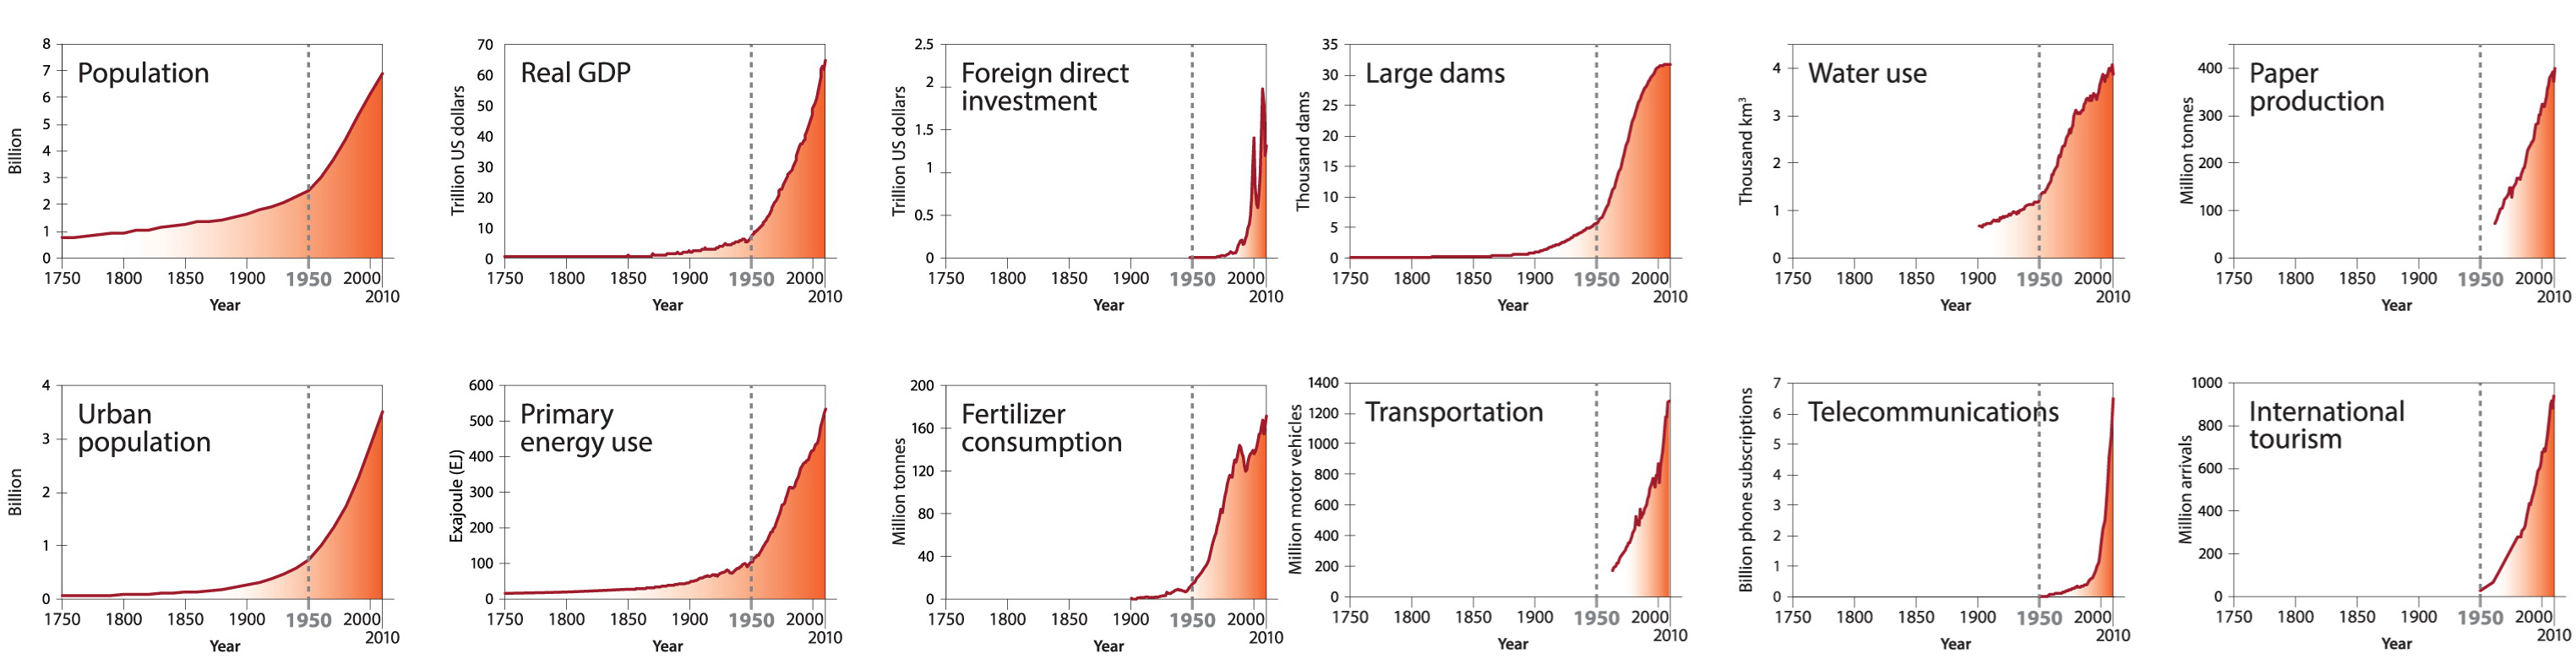
\includegraphics[width=\linewidth]{figures/Anthropocene1V.jpg}
    \caption{Évolution, de 1750 à 2010, de différents indicateurs mondiaux
    du développement socio-économique\cite{steffen_trajectory_2015}.}
    \label{fig:anthropocene1}
\end{figure}
 
\begin{figure}[htbp]
    \centering
    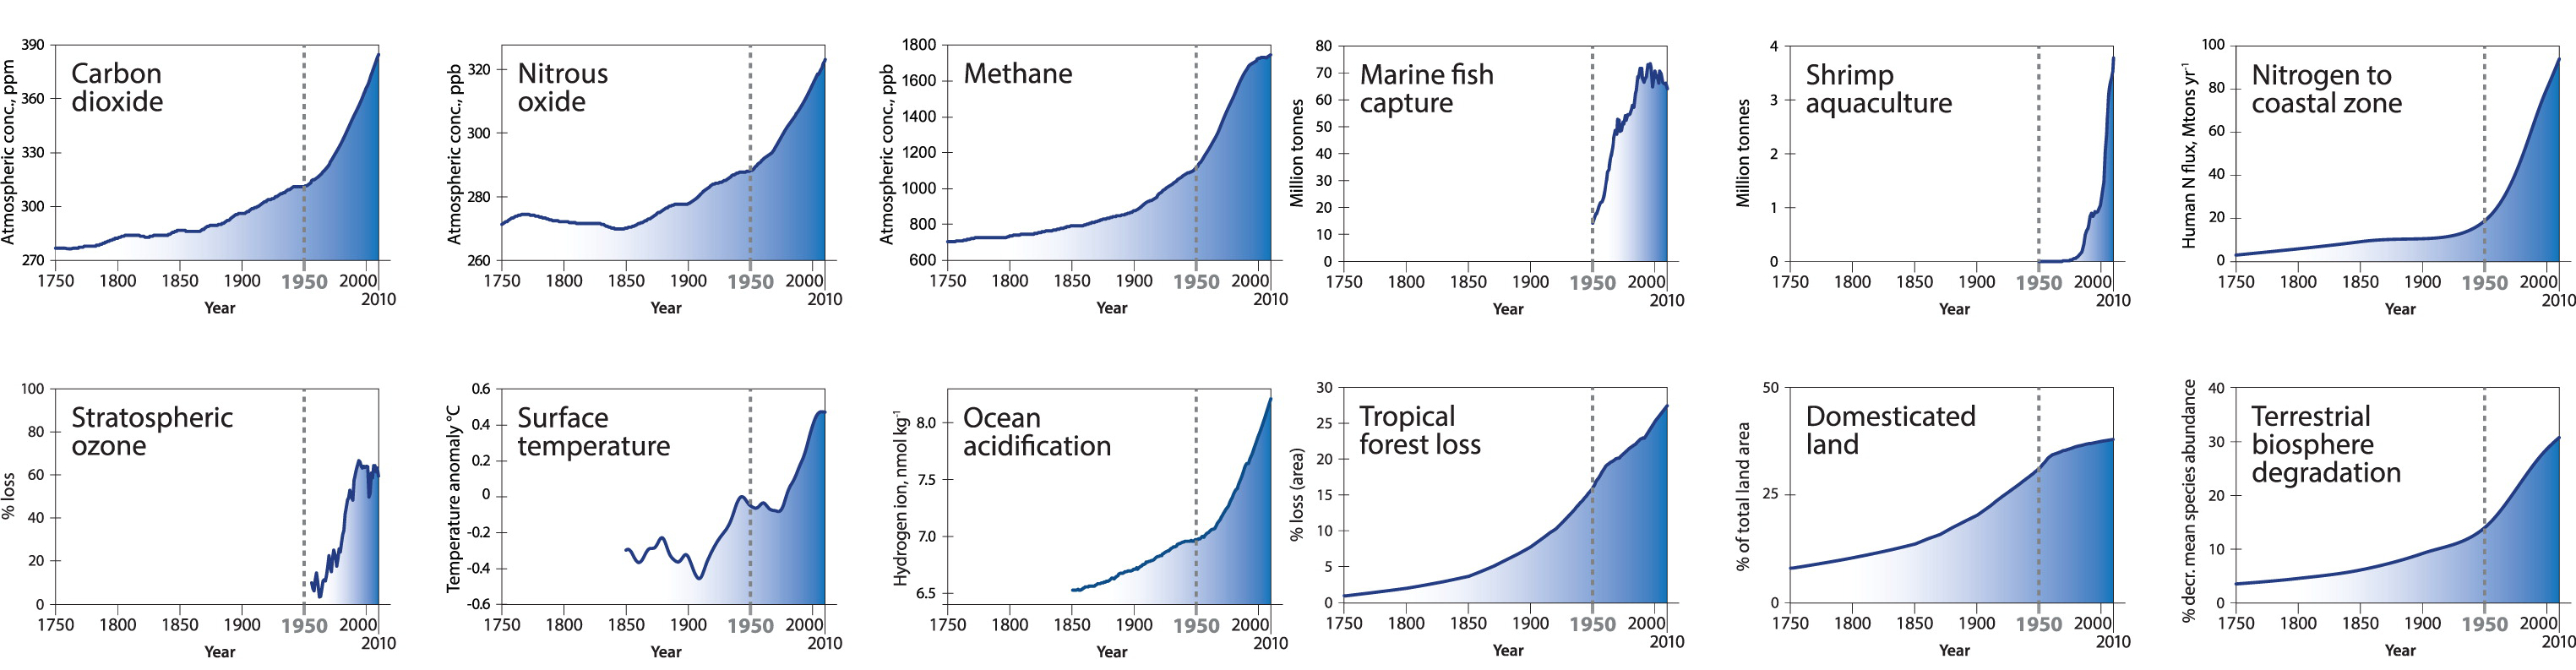
\includegraphics[width=\linewidth]{figures/Anthropocene2V.jpg}
    \caption{Évolution, de 1750 à 2010, de différents indicateurs du
    système terrestre\cite{steffen_trajectory_2015}.}
    \label{fig:anthropocene2}
\end{figure}
 
Ces deux séries présentent la même allure : une évolution lente jusqu'au milieu du \textsc{xx}\textsuperscript{e}~siècle, puis une envolée brutale à partir des années 1950. Cette simultanéité, que les auteurs nomment la \emph{Grande Accélération}, met en évidence le lien direct entre la croissance des activités humaines et la dégradation du système terrestre.

\chapter{Dérèglement climatique}
\section{L'effet de serre}
\label{chap:effet-serre}
\subsection*{La loi de Stefan - Boltzmann}
Pour rappel, les corps rayonnent en fonction de leur température\footfullcite{stefan1879}:
\begin{equation}
  P = \sigma T^4
\end{equation}
avec $P$ la puissance surfacique (W/m$^2$), $\sigma$ la constante de Stefan - Boltzmann (W/m$^2$.K$^4$) et $T$ la température (K).

\subsection*{Mécanisme de l'effet de serre}
Le mécanisme de l'effet de serre peut se décomposer en plusieurs étapes \footfullcite{oce}, \footfullcite{reveilleur-effet-serre}, \footfullcite{ipcc_climate_2021} et est illustré dans la figure \ref{fig:serre}.
\begin{enumerate}
  \item \textbf{Rayonnement venant du Soleil} : le rayonnement solaire atteint le haut de l'atmosphère.
  \item \textbf{Traversée de l'atmosphère terrestre} : une partie du rayonnement est réfléchie vers l'espace, une autre est transmise vers la surface de la Terre.
  \item \textbf{Arrivée à la surface de la Terre} : une partie du rayonnement est réfléchie vers l'atmosphère, l'autre est absorbée par la surface.
  \item \textbf{Accumulation d'énergie} : la température de la surface terrestre augmente car elle reçoit l'énergie du Soleil.
  \item \textbf{Émission de rayonnement infrarouge} : la surface émet alors un rayonnement infrarouge, qui transporte de la chaleur vers l'atmosphère, ce qui refroidit la surface de la Terre.
  \item \textbf{Effet de serre} : certains gaz de l'atmosphère absorbent une partie du rayonnement infrarouge, empêchant que toute la chaleur de ce rayonnement ne s'échappe dans l'espace.
  \item \textbf{Nouvelle absorption par la surface} : la surface de la Terre se réchauffe alors davantage.
\end{enumerate}

\begin{figure}[h]
    \centering
    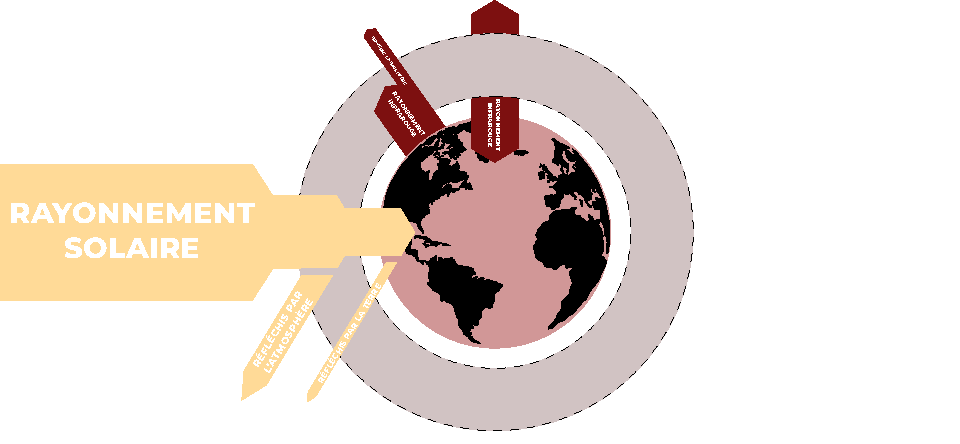
\includegraphics[width=1\linewidth]{figures/serre.pdf}
    \caption{Schéma de principe de l'effet de serre}
    \label{fig:serre}
\end{figure}

La Terre, plus froide que le Soleil, rayonne dans l'infrarouge. Sans effet de serre, la température de la Terre serait à l'équilibre autour de $-18$\,°C. Avec l'effet de serre, la température de la Terre s'équilibre autour de 15\,°C.

Ainsi, l'effet de serre n'est ni « bon » ni « mauvais » : c'est un mécanisme naturel qui maintient la température moyenne de la surface de la Terre autour de 15\,°C, au lieu d'environ $-18$\,°C. 
Le principal gaz à effet de serre est la vapeur d'eau. Sa quantité dans l'atmosphère est globalement stable depuis des milliers d'années. La partie suivante montre l'impact de l'être humain sur l'augmentation de la quantité de gaz à effet de serre dans l'atmosphère. C'est cette augmentation de gaz à effet de serre qui augmente le forçage radiatif conduisant la Terre à se réchauffer.

Les gaz à effet de serre sont simplement définis comme les gaz absorbant le rayonnement infrarouge, c'est une propriété intrinsèque à chaque gaz (certains absorbent le rayonnement infrarouge, d'autres non).

\subsection*{Limite de l'analogie}

\section{Évolution et contribution antropique}

\chapter{Atténuation et Adaptation face au changement climatique}
\section{Atténuation}
\section{Adaptation}
% TODO : à compléter

% =====================================================================
\part{Thermique architecturale}
% =====================================================================

\chapter{Régime dynamique}

\chapter{Enveloppe}

\chapter{Confort}
\label{Confort}

\section{Confort d'hiver}

\section{Confort d'été}
\subsection*{Les brasseurs d'air}
Un brasseur d'air peut fonctionner en mode été ou en mode hiver.
% [Figures : brasseur d'air en mode été / mode hiver]
Pour aller plus loin, voir les études de l'ADEME\footnote{ADEME, \emph{BRASSE : brasseurs d'air, une solution de sobriété et d'efficacité}, 2024 ; ADEME, \emph{BRASSE II : base de données des performances de 50 brasseurs d'air plafonniers à pales}, 2026. \texttt{https://librairie.ademe.fr}}.


\chapter{Équipements}

\section{Ventilation mécanique contrôlée (VMC)}

\section{Chauffage}

\section{Climatisation}

\chapter{Conclusion sur la thermique architecturale}

% =====================================================================
%  Partie 6 -- Cadre réglementaire
% =====================================================================
\part{Cadre réglementaire}
\chapter{Historique}
\chapter{La RE 2020}
\label{chap:re2020}

\section{Introduction}

\subsection*{Objectifs}
La France a adopté un objectif national de neutralité carbone en 2050, instauré par la loi Énergie-Climat (2019), renforcée par la Stratégie nationale bas carbone révisée (2020) et la Programmation pluriannuelle de l'énergie (2020).

Le secteur du bâtiment représente 45\,\% de la consommation énergétique nationale\footnote{ADEME : \texttt{https://www.ademe.fr/les-defis-de-la-transition/batiments} ; Batizoom (ADEME) : \texttt{https://batizoom.ademe.fr}} et 19\,\% des émissions de gaz à effet de serre (associées à l'utilisation de l'énergie)\footnote{ADEME, \emph{op. cit.} ; Xpair : \texttt{https://conseils.xpair.com/analyse\_reglementation/bilan-programme-obec-batiment-energie-carbone.htm}}.

\subsection*{RE et RT}
La France s'est dotée d'une nouvelle réglementation environnementale en 2022, qui prend progressivement la suite de la RT 2012 : la RE 2020.
Nous passons d'une Réglementation Thermique (RT) à une Réglementation Environnementale (RE).

\subsection*{RE 2020}
Elle poursuit des objectifs d'amélioration de la performance énergétique des bâtiments neufs, de réduction de leur impact sur le climat (prise en compte des émissions de gaz à effet de serre sur l'ensemble du cycle de vie des bâtiments) et de leur adaptation aux conditions climatiques futures (renforcement du confort d'été)\footnote{Guide de la RE2020 : \texttt{https://rt-re-batiment.developpement-durable.gouv.fr/IMG/pdf/guide\_re\_2020\_16mai2025.pdf}}.

Elle amène à une amélioration de la conception bioclimatique des bâtiments, elle renforce la performance de l'enveloppe du bâti, elle favorise le recours aux énergies renouvelables et peu carbonées et aux matériaux ayant une faible empreinte carbone.

\subsection*{Catégories et indicateurs}
La RE 2020 s'articule autour de trois catégories (carbone, énergie, confort d'été) et de six indicateurs (tableau \ref{tab:re2020-indicateurs}).

\begin{table}[htbp]
\centering
\caption{Les six indicateurs de la RE 2020}
\label{tab:re2020-indicateurs}
\small
\begin{tabular}{|p{1.6cm}|p{2.6cm}|p{3.8cm}|p{6cm}|}
\hline
\textbf{Catégorie} & \textbf{Indicateur} & \textbf{Définition} & \textbf{Description} \\
\hline
Carbone & $I_c$ construction (kgeqCO$_2$/m$^2$) & Impact sur le changement climatique associé aux « composants » + « chantier » & Introduction de la méthode d'analyse de cycle de vie pour l'évaluation des émissions de gaz à effet de serre des produits de construction et équipements et de leur mise en œuvre : « composants » et « chantier ». \\
\hline
Carbone & $I_c$ énergie (kgeqCO$_2$/m$^2$) & Impact sur le changement climatique associé aux consommations d'énergie primaire & Introduction de la méthode d'analyse de cycle de vie pour l'évaluation des émissions de gaz à effet de serre des énergies consommées pendant le fonctionnement du bâtiment, soit 50 ans. \\
\hline
Énergie & $C_{ep}$ (kWhep/(m$^2$.an)) & Consommation d'énergie primaire totale & Évaluation des consommations d'énergie renouvelable et non renouvelable pour : chauffage, refroidissement, ECS, éclairage, ventilation, éclairage et ventilation des parkings, éclairage des circulations en collectif, électricité des ascenseurs. \\
\hline
Énergie & $C_{ep,nr}$ (kWhep/(m$^2$.an)) & Consommation d'énergie primaire non renouvelable & Idem, pour la seule part non renouvelable. \\
\hline
Énergie & $B_{bio}$ (points) & Besoins bioclimatiques & Évaluation des besoins de chaud, de froid (que le bâtiment soit climatisé ou pas) et d'éclairage. \\
\hline
Confort d'été & DH (°C.h) & Degrés-heures d'inconfort : niveau d'inconfort perçu par les occupants sur l'ensemble de la saison chaude & Évaluation des écarts entre la température du bâtiment et une température de confort (température adaptée en fonction des températures des jours précédents, elle varie entre 26 et 28\,°C). \\
\hline
\end{tabular}
\end{table}

\subsection*{Progressivité}
La RE 2020 prévoit plusieurs phases de renforcement des critères carbone et énergie, en 2025, 2028 puis 2031.

La RE 2020 est entrée en vigueur le 1\textsuperscript{er} janvier 2022 pour les maisons individuelles et les logements collectifs, puis elle a progressivement intégré différents usages.
À partir du 1\textsuperscript{er} mai 2026, quasiment tous les programmes de constructions neuves sont concernés.

\section{Carbone}

\subsection*{Analyse du cycle de vie (ACV)}
L'\textbf{analyse du cycle de vie} (\textbf{ACV}) est une méthode d'évaluation permettant de réaliser un bilan environnemental \textbf{multicritère} d'un système (produit, service ou procédé) sur \textbf{l'ensemble de son cycle de vie} : extraction des matières premières, fabrication, transport, distribution, utilisation, fin de vie, valorisation.
% [Figure : cycle de vie]

\subsection*{L'unité fonctionnelle}
La norme ISO 14044 définit l'unité fonctionnelle comme la « performance quantifiée d'un système de produits, destinée à être utilisée comme unité de référence dans une ACV ».

En ACV, on ne compare pas des objets : on compare la même fonction rendue par des objets ou systèmes différents.
L'unité fonctionnelle est la traduction mesurable de cette fonction.

\subsection*{FDES}
Une Fiche de Déclaration Environnementale et Sanitaire (FDES) est une déclaration environnementale normée. Elle contient les résultats de l'analyse de cycle de vie d'un produit ainsi que des informations sanitaires.
Les FDES sont accessibles sur la base INIES : \texttt{https://base-inies.fr/consultation/recherche}.

\subsection*{$I_c$ projet}
L'impact carbone d'un projet se décompose comme indiqué au tableau \ref{tab:ic-projet} (exemple pour des bureaux).

\begin{table}[htbp]
\centering
\caption{Décomposition de l'$I_c$ projet (exemple : bureaux)}
\label{tab:ic-projet}
\small
\begin{tabular}{|p{3cm}|l|p{6cm}|c|}
\hline
\textbf{Regroupement} & \textbf{Composante} & \textbf{Contenu} & \textbf{Part} \\
\hline
$I_c$ construction & $I_c$ composant & Produits et équipements de construction & 65\,\% \\
(réglementaire) & $I_c$ chantier & Consommation d'énergie et d'eau sur le site, élimination et traitement des déchets & 3\,\% \\
\hline
$I_c$ énergie (réglementaire) & $I_c$ énergie & Consommation d'énergie & 25\,\% \\
\hline
 & $I_c$ eau & Consommation d'eau & 7\,\% \\
\hline
 & $I_c$ parcelle & Utilisation de la parcelle, arrosage & -- \\
\hline
\end{tabular}
\end{table}
$I_c$ bâtiment = $I_c$ construction + $I_c$ énergie + $I_c$ eau ; $I_c$ projet = $I_c$ bâtiment + $I_c$ parcelle.

\subsection*{$I_c$ construction}
L'$I_c$ construction (kgeqCO$_2$/m$^2$) représente l'impact de la construction sur le changement climatique : matériaux et équipements + chantier. Il doit respecter :
\begin{equation}
  I_{c,\mathrm{construction}} \leq I_{c,\mathrm{construction},\mathrm{maxmoyen}} \times \left(1 + Mi_{\mathrm{combles}} + Mi_{\mathrm{surf}}\right) + Mi_{\mathrm{infra}} + Mi_{\mathrm{vrd}} + Mi_{\textrm{géo}} + Mi_{\mathrm{ded}}
\end{equation}
Le seuil moyen est évolutif. Les modulations sont les suivantes :
\begin{itemize}
  \item \textbf{Combles} : permet d'ajuster les exigences pour prendre en compte les surfaces construites non habitables ($h < 1{,}80$\,m).
  \item \textbf{Surface} : permet d'équilibrer les efforts entre petits et grands bâtiments (moyenne : $-30$\,kgCO$_2$e/m$^2$).
  \item \textbf{Infrastructure} : permet d'ajuster les exigences pour prendre en compte les contraintes nécessitant d'importantes fondations ou des espaces souterrains (moyenne : 45\,kgCO$_2$e/m$^2$).
  \item \textbf{VRD} : permet d'ajuster les exigences pour tenir compte des impacts élevés liés à la présence de réseaux d'alimentation du bâtiment ou d'aires de stationnement qui desservent le bâtiment (moyenne : 6\,kgCO$_2$e/m$^2$).
  \item \textbf{Géographie} : permet d'ajuster les exigences pour tenir compte de la mise en œuvre de moyens supplémentaires pour assurer le confort estival du pourtour et de l'arrière-pays méditerranéens.
  \item \textbf{DED} : permet d'ajuster les exigences pour prendre en compte le manque de disponibilité de données environnementales spécifiques (moyenne : 12\,kgCO$_2$e/m$^2$).
\end{itemize}
Source : Observatoire de la RE2020 -- Hub bas carbone -- IFPEB.

\begin{table}[htbp]
\centering
\caption{Seuils $I_{c,\mathrm{construction},\mathrm{maxmoyen}}$ (kgCO$_2$e/m$^2$)}
\label{tab:ic-construction-seuils}
\begin{tabular}{|l|c|c|c|c|}
\hline
\textbf{Usage} & \textbf{2022} & \textbf{2025} & \textbf{2028} & \textbf{2031} \\
\hline
Logement & 740 & 650 & 580 & 490 \\
Bureau & 980 & 810 & 710 & 600 \\
Enseignement primaire et secondaire & 900 & 770 & 680 & 590 \\
\hline
\end{tabular}
\end{table}

\subsection*{$I_c$ énergie}
L'$I_c$ énergie (kgeqCO$_2$/m$^2$) représente l'impact de l'énergie sur le changement climatique (consommation d'énergie et d'eau). Il doit respecter :
\begin{equation}
  I_{c,\textrm{énergie}} \leq I_{c,\textrm{énergie},\mathrm{maxmoyen}} \times \left(1 + Mi_{\mathrm{combles}} + Mi_{\mathrm{surf\_moy}} + Mi_{\mathrm{surf\_tot}} + Mi_{\mathrm{cat}} + Mi_{\textrm{géo}}\right)
\end{equation}
Les seuils moyens sont évolutifs et donnés par le gouvernement par typologie de programme. Les modulations sont les suivantes :
\begin{itemize}
  \item \textbf{Combles} : permet d'ajuster les exigences pour prendre en compte les surfaces construites non habitables ($h < 1{,}80$\,m).
  \item \textbf{Surface} : permet d'équilibrer les efforts entre petits et grands bâtiments.
  \item \textbf{Surface totale} : modulation spécifique pour les logements collectifs pour équilibrer les efforts liés aux parties collectives entre petits et grands collectifs.
  \item \textbf{Contraintes} : permet de compenser les contraintes extérieures qui limitent les possibilités de ventilation naturelle du bâtiment par ouverture des fenêtres.
  \item \textbf{Géographie} : permet d'ajuster les exigences pour tenir compte de la mise en œuvre de moyens supplémentaires pour assurer le confort estival du pourtour et de l'arrière-pays méditerranéens.
\end{itemize}

\begin{table}[htbp]
\centering
\caption{Seuils $I_{c,\textrm{énergie},\mathrm{maxmoyen}}$ (kgCO$_2$e/m$^2$)}
\label{tab:ic-energie-seuils}
\begin{tabular}{|l|c|c|c|}
\hline
\textbf{Usage} & \textbf{2022} & \textbf{2025} & \textbf{2028} \\
\hline
Logement & 560 & 320 & 260 \\
Bureau & 280 & 200 & -- \\
Enseignement primaire et secondaire & 240 & 200 & 140 \\
\hline
\end{tabular}
\end{table}

\subsection*{Un outil en ligne pour l'ACV et l'$I_c$}
Décarbone+ (AIA Environnement) : \texttt{https://www.decarbone-plus.com/}

\section{Énergie}

\subsection*{Énergie primaire}
L'énergie primaire est une forme d'énergie disponible dans la nature avant toute transformation.

En France, la consommation d'énergie primaire s'élève à 2\,630\,TWh en 2024 (donnée corrigée des variations climatiques)\footnote{\texttt{https://www.statistiques.developpement-durable.gouv.fr/}}, répartie en :
\begin{itemize}
  \item 41\,\% de nucléaire ;
  \item 28\,\% de pétrole ;
  \item 12\,\% de gaz naturel ;
  \item 17\,\% d'énergies renouvelables et déchets (dont 1\,\% de déchets non renouvelables) ;
  \item 2\,\% de charbon.
\end{itemize}
% [Figure : évolution de la consommation d'énergie primaire 1990-2024]

\subsection*{Consommation d'énergie primaire}
La consommation d'énergie primaire $C_{ep}$ (kWhep/(m$^2$.an)) doit respecter :
\begin{equation}
  C_{ep} \leq C_{ep,\mathrm{maxmoyen}} \times \left(1 + Mi_{\mathrm{combles}} + Mi_{\mathrm{surf\_moy}} + Mi_{\mathrm{surf\_tot}} + Mi_{\mathrm{cat}} + Mi_{\textrm{géo}}\right)
\end{equation}
Les modulations sont les mêmes que pour l'$I_c$ énergie (combles, surface, surface totale, contraintes, géographie).

\subsection*{Consommation d'énergie primaire non renouvelable}
De même, la consommation d'énergie primaire non renouvelable $C_{ep,nr}$ (kWhep/(m$^2$.an)) doit respecter :
\begin{equation}
  C_{ep,nr} \leq C_{ep,nr,\mathrm{maxmoyen}} \times \left(1 + Mi_{\mathrm{combles}} + Mi_{\mathrm{surf\_moy}} + Mi_{\mathrm{surf\_tot}} + Mi_{\mathrm{cat}} + Mi_{\textrm{géo}}\right)
\end{equation}

\begin{table}[htbp]
\centering
\caption{Seuils de consommation d'énergie primaire (kWhep/(m$^2$.an))}
\label{tab:cep-seuils}
\begin{tabular}{|l|c|c|}
\hline
\textbf{Usage} & \textbf{$C_{ep,\mathrm{maxmoyen}}$} & \textbf{$C_{ep,nr,\mathrm{maxmoyen}}$} \\
\hline
Logement & 85 & 70 \\
Bureau & 85 & 75 \\
Enseignement primaire et secondaire & 72 & 65 \\
\hline
\end{tabular}
\end{table}

\subsection*{Besoin bioclimatique conventionnel}
Le calcul du $B_{bio}$ RE2020 comprend les besoins en chauffage, en refroidissement et en éclairage du bâtiment.
Le $B_{bio}$ s'intéresse uniquement au bâti et non aux équipements.

Le $B_{bio}$ s'intéresse à :
\begin{itemize}
  \item l'orientation ;
  \item l'isolation ;
  \item la compacité ;
  \item les surfaces vitrées ;
  \item la protection solaire ;
  \item l'inertie ;
  \item la conception globale de l'enveloppe.
\end{itemize}

Le $B_{bio}$ (en points) doit respecter :
\begin{equation}
  B_{bio} \leq B_{bio,\mathrm{maxmoyen}} \times \left(1 + Mi_{\mathrm{combles}} + Mi_{\mathrm{surf\_moy}} + Mi_{\mathrm{surf\_tot}} + Mi_{\mathrm{bruit}} + Mi_{\textrm{géo}}\right)
\end{equation}
Les modulations sont : combles, surface, surface totale, géographie (comme précédemment), et \textbf{bruit} : coefficient de modulation selon l'exposition au bruit des infrastructures de transport à proximité du bâtiment.

\section{Confort d'été}

\subsection*{Degrés-heures d'inconfort}
Le calcul des degrés-heures d'inconfort (DH) suit les étapes suivantes :
\begin{enumerate}
  \item météo avec scénario caniculaire, en fonction de la zone climatique ;
  \item calcul en mode confort d'été (simulation avec un logiciel spécialisé) ;
  \item somme des degrés-heures ;
  \item comparaison du DH du projet au DH$_{\max}$.
\end{enumerate}

Chaque heure, on compte l'écart entre la température du bâtiment et la température limite de confort (lorsque la première dépasse la seconde). Par exemple, pour une journée type d'été en occupation, avec un seuil à 27\,°C (température extérieure moyenne des jours passés haute), le cumul de la journée atteint 20,0\,°C.h.
% [Figure : journée type d'été en occupation]

\subsection*{Seuils}
\begin{itemize}
  \item \textbf{Catégorie 1} : situation à moindre contrainte extérieure, ainsi que les bâtiments non climatisés (sauf parties de bâtiments climatisées en zones H2d et H3).
  \item \textbf{Catégorie 1 climatisée} : pour les zones H2d et H3.
  \item \textbf{Catégorie 2} : situation de contrainte forte. Les bâtiments doivent être localisés dans une région « chaude » à faible altitude, climatisés et exposés à des nuisances sonores.
  \item \textbf{Catégorie 3} : situation de contrainte très forte, uniquement pour les bureaux climatisés soumis à des règles interdisant l'ouverture des fenêtres et les immeubles de grande hauteur.
\end{itemize}

\begin{table}[htbp]
\centering
\caption{Seuils de degrés-heures d'inconfort DH$_{\max}$ (°C.h)}
\label{tab:dh-seuils}
\small
\begin{tabular}{|p{4.2cm}|c|c|c|c|}
\hline
\textbf{Usage} & \textbf{Cat. 1} & \textbf{Cat. 1 clim.} & \textbf{Cat. 2} & \textbf{Cat. 3} \\
\hline
Logement, $S_{moy} \leq 20$\,m$^2$ & 1250 & 1600 & 2600 & -- \\
Logement, $20 < S_{moy} \leq 60$\,m$^2$ & 1250 & $1700 - 5\times S_{moy}$ & $2850 - 12{,}5\times S_{moy}$ & -- \\
Logement, $S_{moy} > 60$\,m$^2$ & 1250 & 1400 & 2100 & -- \\
\hline
Bureau & 1150 & 2400 & 2600 & pas de seuil \\
\hline
Enseignement primaire et secondaire & 900 & 1800 & 2200 & -- \\
\hline
\end{tabular}
\end{table}

% =====================================================================
\part{Conclusion et perspectives}
% =====================================================================

\chapter{Synthèse}

Ce cours a présenté les bases physiques de la thermique du bâtiment. La chaleur se transmet via les trois modes de transferts de chaleur qui sont la conduction, la convection et le rayonnement.
L'air est humide, il contient de la vapeur d'eau qui migre à travers les parois et peut condenser dès qu'elle atteint son point de rosée.

L'architecte n'a pas besoin de savoir résoudre les équations présentées dans ce cours. En revanche, il doit en comprendre les mécanismes pour faire des choix en phase de conception : implantation, orientation, volumétrie, composition des parois, dessin des détails. Ce sont ces choix architecturaux, qui déterminent le confort des usagers, la consommation d'énergie et l'impact carbone du projet. Les équipements (chauffage, ventilation, climatisation) viennent ensuite compléter une conception déjà performante (et non compenser des erreurs ou oublis de conception.

\chapter{Interventions}

\section{Projet neuf}

En projet neuf, l'architecte dispose de beaucoup de liberté. Voici les principales questions à se poser, à peu près dans l'ordre où elles apparaissent dans le projet :

\begin{enumerate}
    \item \textbf{Le site et le climat} : quel est le climat local ? D'où vient le soleil ? Quels sont les masques (bâtiments voisins, végétation, relief) ?
    \item \textbf{L'implantation et l'orientation} : orienter le bâtiment pour capter les apports solaires en hiver et pouvoir s'en protéger en été. Le choix de l'emplacement des espaces tampons
    \item \textbf{La volumétrie} : privilégier une volumétrie compacte, qui limite la surface d'enveloppe en contact avec l'extérieur, et donc les déperditions.
    \item \textbf{Les ouvertures} : dimensionner et répartir les surfaces vitrées selon l'orientation, et prévoir dès l'esquisse les protections solaires extérieures (casquettes, brise-soleil, volets, végétation).
    \item \textbf{L'enveloppe} : choisir une stratégie d'isolation continue et dessiner les détails pour traiter les ponts thermiques (jonctions mur/plancher, balcons, menuiseries). Assurer l'étanchéité à l'air.
    \item \textbf{La gestion de la vapeur} : ordonner les couches des parois pour que leur perméabilité à la vapeur augmente de l'intérieur vers l'extérieur, ou prévoir une membrane adaptée. Vérifier le comportement des parois en hiver et en été (avec Ubakus par exemple).
    \item \textbf{L'inertie et la ventilation} : conserver de la masse côté intérieur et permettre la ventilation naturelle traversante, notamment la nuit en été. Prévoir le renouvellement d'air et l'évacuation de l'humidité des pièces humides.
    \item \textbf{Les matériaux} : privilégier des matériaux à faible impact carbone (biosourcés, géosourcés, réemploi) en s'appuyant sur les FDES.
    \item \textbf{La réglementation} : garder en tête les six indicateurs de la RE 2020, en dialogue avec le bureau d'études thermiques. Le $B_{bio}$, le $I_c Construction$ et les degrés-heures d'inconfort dépendent directement des choix  de l'architecte.
\end{enumerate}

\section{Projet de réhabilitation}

En réhabilitation, le bâtiment existe déjà : son orientation, sa volumétrie et une partie de ses matériaux sont imposés par l'existant. La RE 2020 ne s'applique pas (pour le moment...), mais les enjeux de confort, d'énergie et de carbone restent les mêmes. Réhabiliter plutôt que démolir est d'ailleurs le choix le plus sobre en carbone. Voici les principales questions à se poser :

\begin{enumerate}
    \item \textbf{Le diagnostic} : avant toute intervention, comprendre comment le bâtiment fonctionne. De quoi sont faits les murs ? Comment gèrent-ils l'humidité ? Y a-t-il des désordres (humidité, moisissures, fissures) ? Où sont les principales déperditions ?
    \item \textbf{Les priorités} : intervenir d'abord là où les pertes sont les plus importantes. (La toiture, les murs,les menuiseries, le plancher bas.)
    \item \textbf{La stratégie d'isolation} : choisir entre isolation par l'extérieur (plus performante, conserve l'inertie, mais modifie la façade) et isolation par l'intérieur (préserve la façade, notamment patrimoniale, mais crée des ponts thermiques et réduit la surface habitable).
    \item \textbf{Le respect des murs anciens} : les murs anciens (pierre, brique, pisé, pan de bois) fonctionnent souvent grâce à leur capacité à laisser migrer la vapeur et à sécher. Les isoler avec des matériaux ou des membranes inadaptés peut piéger l'humidité et provoquer des désordres importants. Il s'agit de privilégier des matériaux perspirants (fibre de bois, chanvre, enduits à la chaux ou à la terre).
    \item \textbf{Les ponts thermiques} : identifier ceux que l'intervention ne pourra pas supprimer (planchers, refends, balcons) et vérifier qu'ils ne provoqueront pas de condensation de surface.
    \item \textbf{La ventilation} : une enveloppe rénovée est souvent plus étanche à l'air. Il peut être necessaire de prévoir un renouvellement d'air adapté, (pour éviter que l'humidité provoque de la condensation et moisissures).
    
\end{enumerate}

Dans tous les cas, une réhabilitation se pense de manière globale : intervenir sur un seul élément (changer les fenêtres sans ventiler, isoler sans traiter l'humidité) peut créer plus de problèmes qu'il n'en résout.
\chapter{Pour aller plus loin}
La bibliographie complète est présentée en fin de document, voici ici une liste plus courte de ressources utiles à consulter dans différents format :

\begin{encadre}{Livre}
  \begin{itemize}
    \item \textit{La Thermique du bâtiment}, O. Benjeddou (2016)
  \end{itemize}
\end{encadre}

\begin{encadre}{Site Web}
  \begin{itemize}
    \item AMACO plateforme ressources, \url{https://ressources.amaco.org/}
    \item UBAKUS, \url{https://www.ubakus.de/fr/calculateur-valeur-u/?}
  \end{itemize}
\end{encadre}

\begin{encadre}{Bande dessinés}
  \begin{itemize}
    \item \textit{Le monde sans fin}, Jancovici et Blain (2021)
    \item \textit{Ressources : un défi pour l'humanité}, Bihouix et Perriot (2024)
  \end{itemize}
\end{encadre}

\begin{encadre}{Vidéos}
  \begin{itemize}
    \item \textit{Climatisation : un désastre écologique ?}, \textit{Le Reveilleur}, R.Meyer (2026), \url{https://www.youtube.com/watch?v=nERo6YzNoSM}
  \end{itemize}
\end{encadre}


\backmatter
\printbibliography[heading=bibintoc]   % bibintoc = l'ajoute à la table des matières
\end{document}
